%!TEX root = ../thesis.tex
\documentclass[..thesis.tex]{subfiles}

\begin{document}

This sections describes three different approaches for increasing the sampling frequency for Honest Profiler. To verify the performance overhead of the solution and its accuracy, a benchmark test was executed on each solution.

\subsection{Benchmark}
Benchmark test reads 10000000 random integers from an input file and then performs quicksort on the copy of the obtained list of integer 10 times. All tests are performed on a machine running Intel i5-5200U CPU with 8 GB of RAM.

Baseline of the test using the default implementation of the Honest Profiler finished the test in 74.72 seconds on average. During profiling, 19025 samples were obtained on average from which 15130 (81\%) contained frames of interest.
Profiling results are visualized on the figure ~\ref{fig:baseline} on page ~\pageref{fig:baseline}.
\TODO{Before shipping final, verify that the pictures are positioned well}
\TODO{Is defining test machine specs necessary?}
\TODO{Is it better to move benchmark profiling result visualizations to appendices?}

\begin{figure}[H]
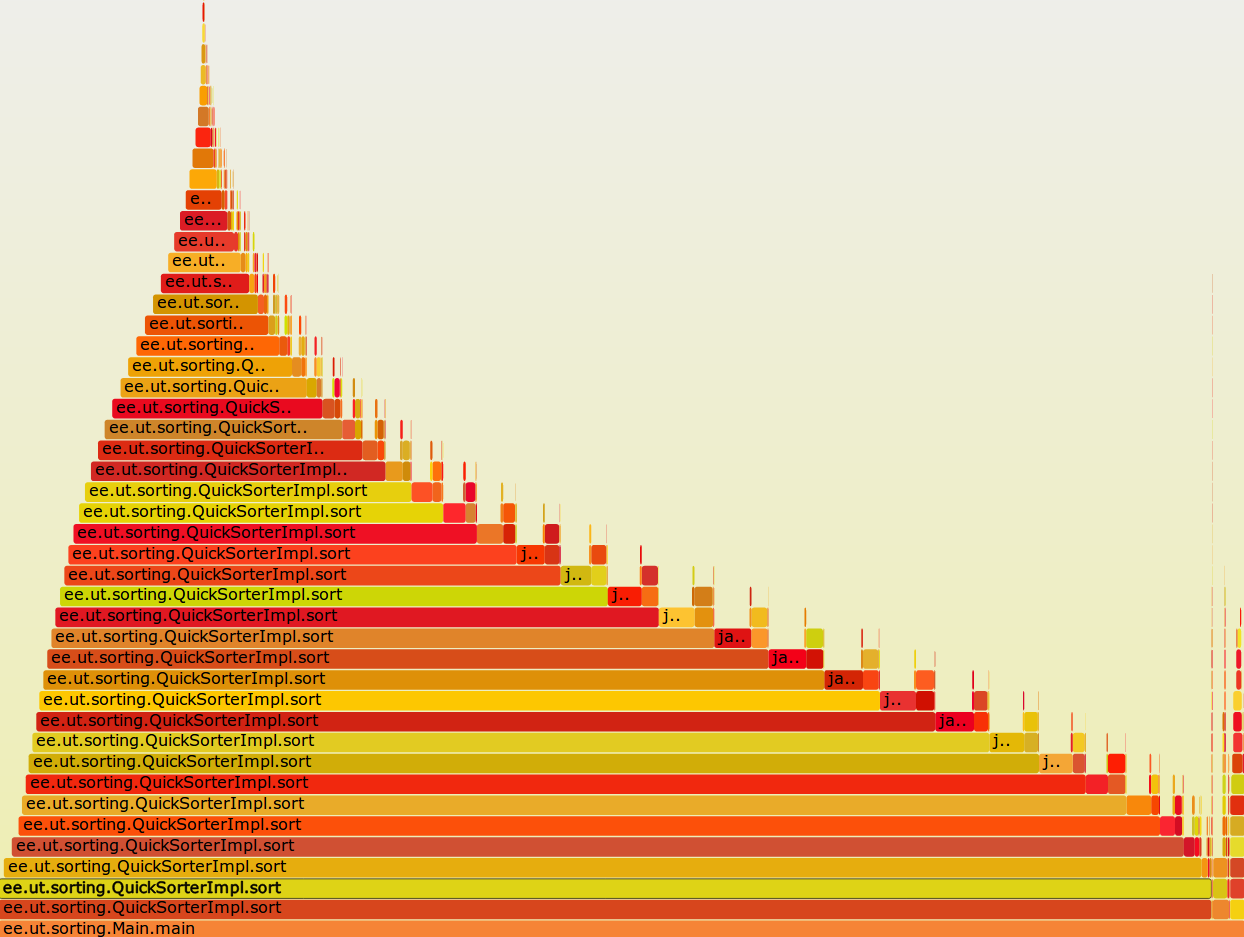
\includegraphics[scale=0.335]{baseline.png}
\caption{Visualization of baseline benchmark profiling results}
\label{fig:baseline}
\end{figure}

\subsection{Optimization implementations}
This thesis covers three method to obtain more samples from the observable application than it would be for the default implementation of the Honest Profiler. Following sections will describe their implementations more in-depth.

\subsubsection{Interval timer based on real time}
Existing implementation of Honest Profiler uses CPU time based interval timer from GNU time library. Alternative approach would be to use an interval timer which counts time in real time instead. The very same interval timer from GNU time library can be configured in such way that it counts down in real time by initilizing it with \texttt{ITIMER\_REAL} flag in the manner as shown in listing ~\ref{lst:itimer_real}.

\begin{lstlisting}[language=C++,style=def,label={lst:itimer_real}, caption={Timer initialization based on real time}]
#include <sys/time.h>
struct itimerval timer;
setitimer(ITIMER_REAL, &timer, 0)
\end{lstlisting}

Upon timer expiration, a \texttt{SIGALRM} signal is sent to the process.\cite{getitimer2}

Using real time based timer means that its interval is not limited by the system's clock frequency as it would be for CPU time based timers. Due to this fact, the timer can even be configured to send the \texttt{SIGALRM} signal every 1 microsecond.

Although this approach obtains considerably larger amount of samples due to higher profiling frequency, it also introduces a potential bias that could affect the profiling results. It might be possible that between the two consecutive timer expiration signals, the observable application has not received any processor time to perform its instructions. This would imply that the same sample in the exact same state is persisted multiple times. Similar issue occurs the other way around when the application's instructions are executed on multiple processor cores. There is a clear distinction in cases in which 4 processor cores are fully utilized executing the application's instructions and cases in which a single processor core is used. The former scenario would get roughly four times as much work done when compared to the latter scenario. However, the real time based timer will not take therse workload differences into account because it measures time based on the real world clock.

Average benchmark runtime using this method finished in 82.36 seconds and obtained up to 12.8 million samples during its runtime from which only 73982 (0.58\%) contained frames of interest. Whereas the 10\% increase in execution times is acceptable for gaining significantly larger amount of samples, it is unknown why only 0.58\% of the gathered samples contained frames of interest. This phenomenom is also further covered in the future research section ~\ref{sec:future-research}. Visualization of the profiling results utilizing this method can be observed in figure ~\ref{fig:walltime} on page ~\pageref{fig:walltime}.
\begin{figure}[H]
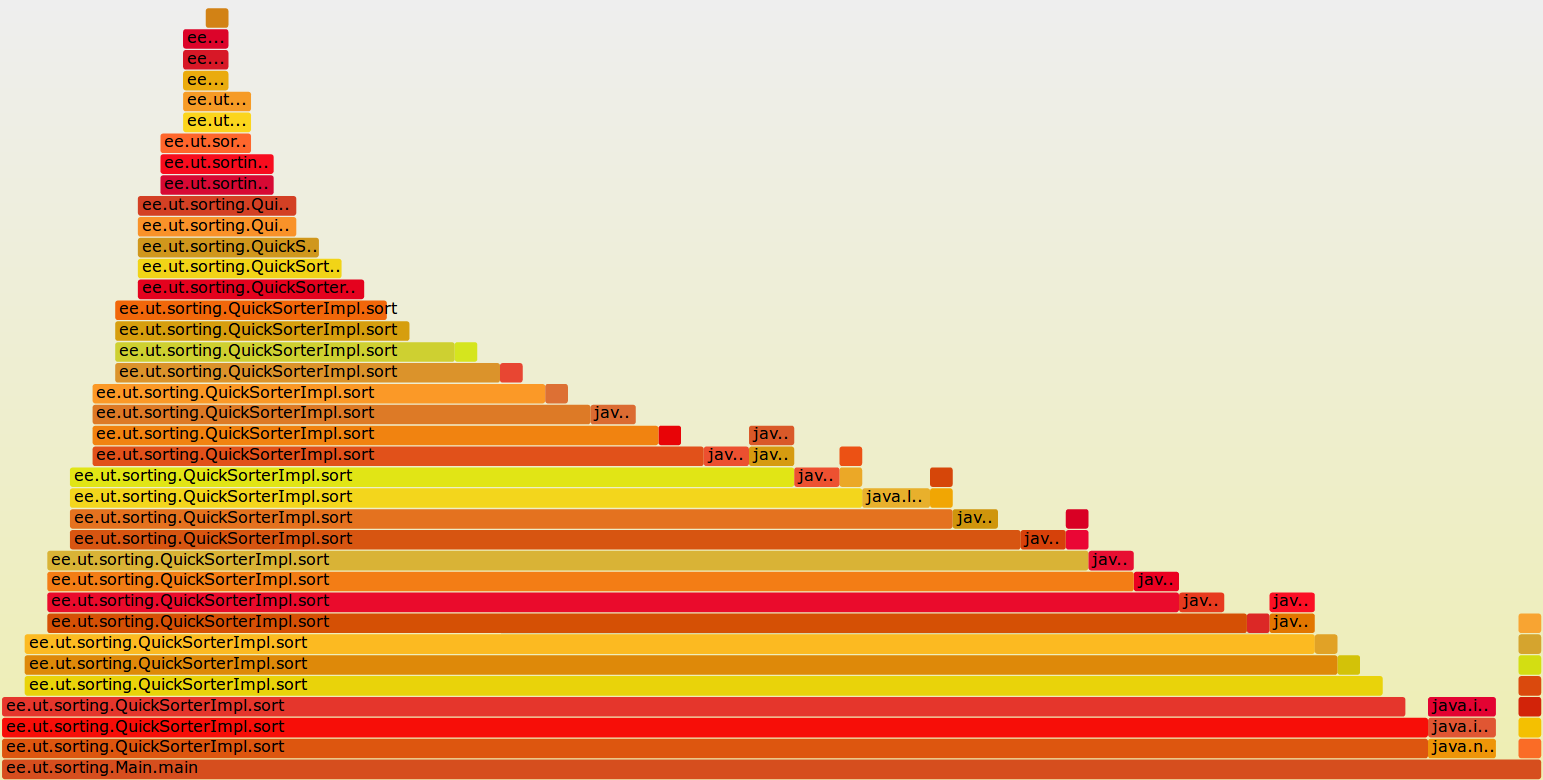
\includegraphics[scale=0.27]{walltime.png}
\caption{Visualization of real time based solution profiling results}
\label{fig:walltime}
\end{figure}

\subsubsection{Increasing the kernel clock frequency}
As CPU time based interval timer from GNU timer library is directly dependent on the kernel's internal timer frequency, one approach to gather more samples to build a custom kernel with increased kernel clock frequency. By default this frequency is set to 250 Hz.\cite{torvalds_linux:_2018} This value can be increased to achieve higher sampling frequency. 

This can be accomplished by creating a custom configuration in the \texttt{Kconfig.hz} with a desired frequency value and building the kernel using the created configuration. An easier way to obtain a kernel with higher kernel timer frequency would be to install a \texttt{linux-lowlatency} kernel package which has set the kernel timer frequency to 1000 Hz.

Using the 1000 Hz kernel increases the sampling frequency as the CPU time based interval timer from GNU time library can now send an interrupt signal every $\frac{1}{1000} = 0.001$ seconds. Experiments with such kernel has shown four times increase in the amount of samples gathered wihtout causing significant performance overhead to the observable application.

Benchmark runs on such configuration had average runtime of 77.33 seconds during which 70525 samples were collected. 50937 of the samples (72\%) consisted of meaningful samples. Visualization from a runtime using such profiling configuration is shown on figure ~\ref{fig:hz_increase} on page ~\pageref{fig:hz_increase}.
\begin{figure}[H]
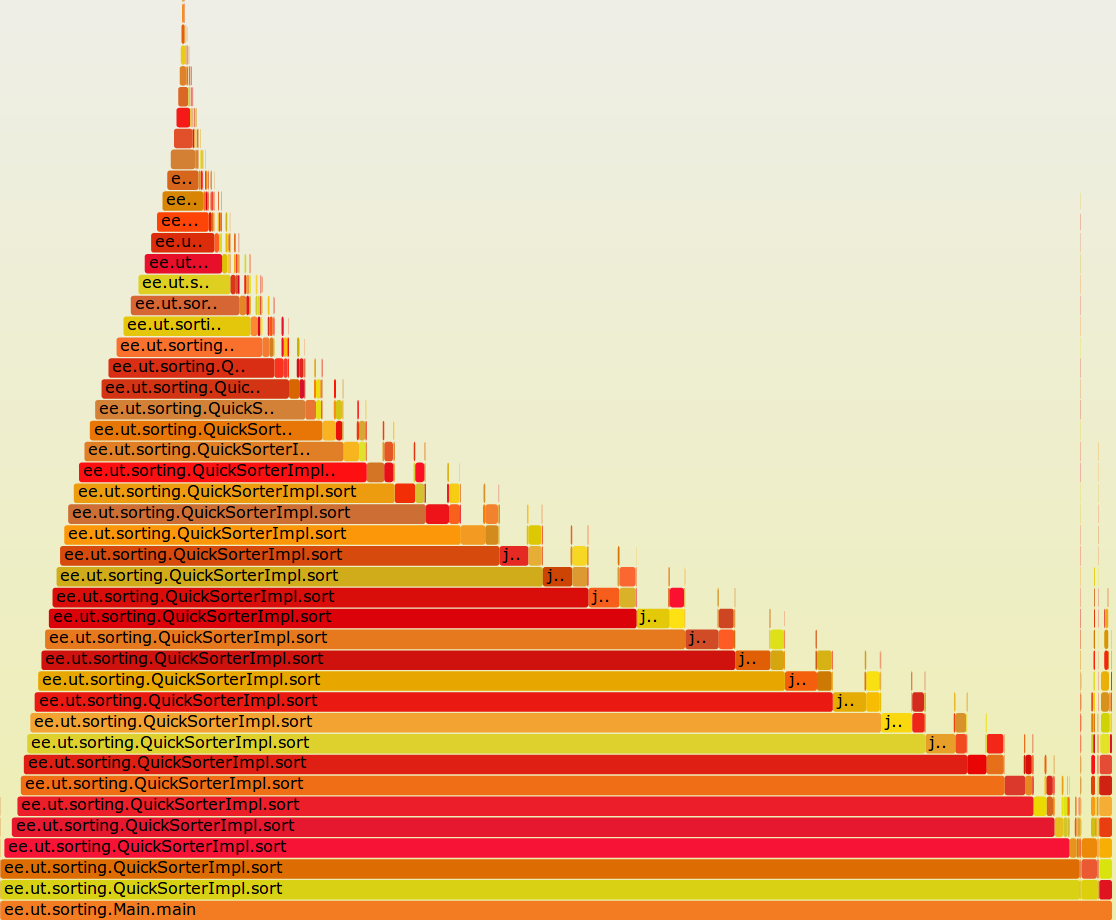
\includegraphics[scale=0.375]{hz_increase.png}
\caption{Visualization of the results from profiling with increased kernel timer frequency}
\label{fig:hz_increase}
\end{figure}

\subsubsection{External utility for timekeeping}
\label{shared-mem}

This approach moves the time measurement logic to an external server process which uses UNIX operating system signals and shared memory to communicate with Honest Profiler and the profileable Java process. The solution is based on the fact that it is possible for a process to obtain the CPU time that the process has used without the limitations imposed by the kernel's internal timer frequency. The CPU time spent by a process can be obtained by calling the \texttt{clock\_\-gettime} function from the GNU time library.

This solution has two benefits over the default implementation of Honest Profiler:
\begin{enumerate}
	\item Extracting the interval timing logic from the Honest Profiler native agent reduces performance overhead caused to the observable Java process
	\item Enables calling \texttt{Async\-Get\-Call\-Trace} method more often than default implementation
\end{enumerate}

The external server process starts by creating an UNIX domain socket and waits for a connection. Upon a connection from the observable Java process with Honest Profiler's native agent attached, it obtains its process identifier (\textit{pid}) for signal sending purposes. The server process then allocates a memory section which is shared with the profileable Java process. Server will then use two signals to request action from the Honest Profiler that is attached to the Java process:
\TODO{Signal handler safety worth mentioning?}
\begin{itemize}
	\item \texttt{SIGALRM} - write the used CPU time used by the Java process to the shared memory
	\item \texttt{SIGPROF} - call the \texttt{Async\-Get\-Call\-Trace} method to obtain a sample from the thread handling the signal
\end{itemize}

Shared memory for interprocess communication is used due to its superior performance over other communication approaches such as file I/O (input/output) or UNIX domain sockets. 

Figure ~\ref{fig:shared_mem_arctitecture} on page ~\pageref{fig:shared_mem_arctitecture} summarizes the architecture of this implementation.

\begin{figure}[H]
\centering
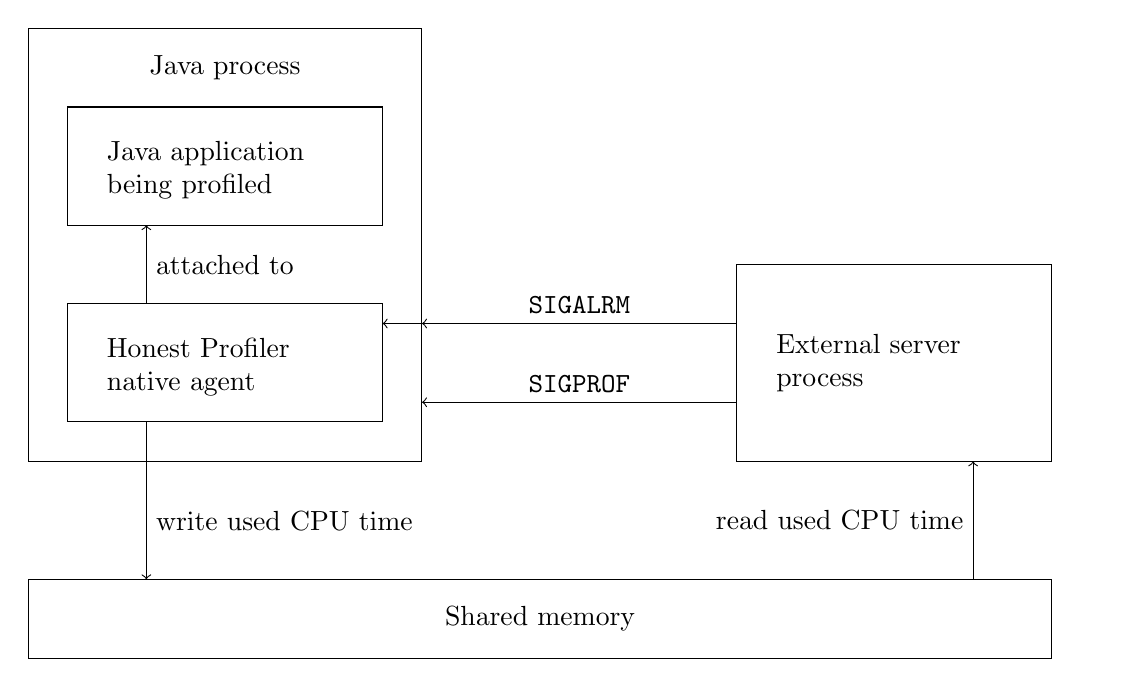
\begin{tikzpicture}
\draw (0,0) rectangle (5,5.5) node at (2.5,5) {Java process};
\draw (0.5,4.5) rectangle (4.5,3) node[text width=4cm] at (3,3.7) {Java application \\being profiled};

\draw (0.5,2.0) rectangle (4.5,0.5) node[text width=4cm] at (3,1.2) {Honest Profiler \\native agent};

\draw (9,0) rectangle (13,2.5) node[text width=4cm] at (11.5,1.25) {External server \\process};

\draw (0,-2.5) rectangle (13,-1.5) node[pos=.5] {Shared memory};

\draw[->] (1.5,2) -- (1.5, 3) node[right, pos=0.5] at (2.6,4.4) {attached to};

\draw[->] (9,1.75) -- (5,1.75) node[above, pos=.5] {\texttt{SIGALRM}};
\draw[->] (5,1.75) -- (4.5,1.75);
\draw[->] (9,0.75) -- (5,0.75) node[above, pos=.5] {\texttt{SIGPROF}};

\draw[->] (1.5,0.5) -- (1.5,-1.5) node[right, pos=0.63] {write used CPU time};
\draw[->] (12,-1.5) -- (12, 0) node[left, pos=0.5] {read used CPU time};


\end{tikzpicture}
\caption{Architecture of the concept}
\label{fig:shared_mem_arctitecture}
\end{figure}

\TODO{sleeping logic to reduce overhead worth mentioning?}

Testing shows that such modification for Honest Profiler runs the benchmark test in 72.16 seconds on average.

\end{document}